\definecolor{lavander}{cmyk}{0,0.48,0,0}
\definecolor{violet}{cmyk}{0.79,0.88,0,0}
\definecolor{burntorange}{cmyk}{0,0.52,1,0}

\def\lav{lavander!90}
\def\oran{orange!30}

\tikzstyle{time}=[draw,circle,violet,bottom color=\lav,
                  top color= white, text=violet,minimum width=20pt]
\tikzstyle{base}=[draw,circle,burntorange, left color=\oran,
                       text=violet,minimum width=20pt]

\begin{figure}[h!]
\centering
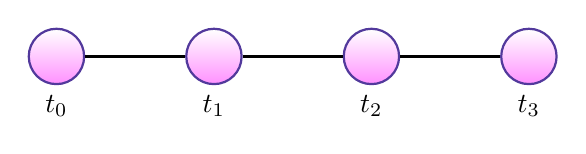
\begin{tikzpicture}[auto, thick]
  \node[time,label=below:$t_0$] (t0) at (0,0) {};
  \node[time,label=below:$t_1$] (t1) at (2,0) {};
  \node[time,label=below:$t_2$] (t2) at (4,0) {};
  \node[time,label=below:$t_3$] (t3) at (6,0) {};
  
  \path (t0) edge (t1);
  \path (t1) edge (t2);
  \path (t2) edge (t3);


\end{tikzpicture}
\caption{Multi-period optimal power flow example with four time-steps. The lines connecting the different time-periods denote the coupling between them.}
\label{fig:tcopflow}
\end{figure}